
\marginpar{\href{https://youtu.be/H_k1w3cfny8}{Video}}
\marginpar{\href{https://ocw.mit.edu/courses/6-041sc-probabilistic-systems-analysis-and-applied-probability-fall-2013/pages/unit-ii/lecture-10/}{Lecture Home}}
\marginpar{\href{https://ocw.mit.edu/courses/6-041sc-probabilistic-systems-analysis-and-applied-probability-fall-2013/b8c5d01b95379ca38ea3057529d253f7_MIT6_041SCF13_L10.pdf}{Slides}}

Reading: 3.6, 4.1

Conditional PDF's are just slices of joint PDF's

\subsection{The Bayes' Variations}

\marginpar{(4m)}

\begin{figure}[h]
\centering
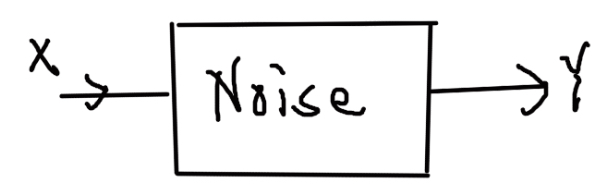
\includegraphics[width=6cm, height=3cm]{images/L10/noise_model.jpeg}
\caption{x}
\end{figure}

\marginpar{(5:45)}

The output of an inference problem is to come up with the distribution of X (unknown quantity) given what we observe.

\subsubsection{Continuous Counterpart}

\begin{align*}
f_{X|Y}(x|y) = \frac{f_{X,Y}(x,y)}{f_Y(y)}  = \frac{f_X(x) f_{Y|X}(y|x)}{f_Y(y)}\\
f_Y(y) = \int_X f_X(x) f_{Y|X}(y,x)dx
\end{align*}

\subsection{Discrete X, Continuous Y}

\marginpar{(10m)}

\begin{figure}[h]
\centering
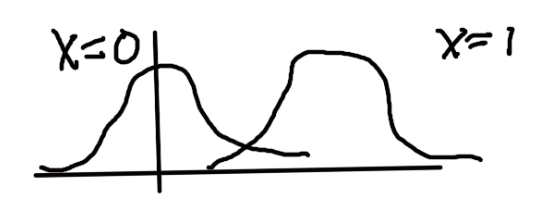
\includegraphics[width=5cm, height=4cm]{images/L10/discrete_continuous.jpeg}
\caption{Discrete X, Continuous Y}
\end{figure}

\subsection{Continuous X, Discrete Y}

\marginpar{(17:50)}

\begin{figure}[h]
\centering
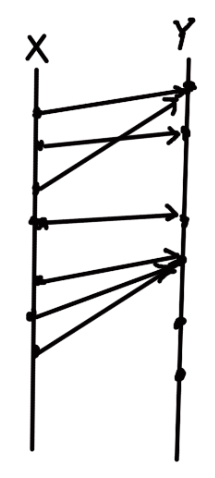
\includegraphics[width=4cm, height=8cm]{images/L10/continuous_discrete.jpeg}
\caption{Continuous X, Discrete Y}
\end{figure}

\subsection{Derived Distribution}

\marginpar{(20:30)}

\subsection{Discrete Case}

\marginpar{(22:45)}

\subsection{Continuous Case}

\marginpar{(23:45)}

\subsection{Two-step Procedure}

\marginpar{(26:10)}

\subsection{Example: Joan drives from Boston to NY}

\marginpar{(32:45)}

\begin{figure}[h]
\centering
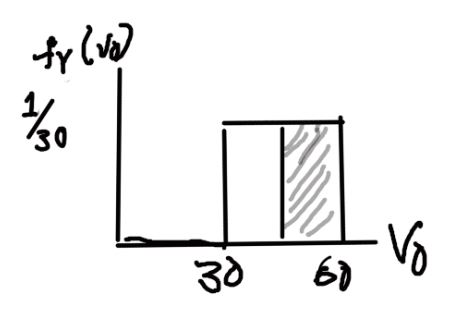
\includegraphics[width=5cm, height=4cm]{images/L10/joan_drives.jpeg}
\caption{x}
\end{figure}

\subsection{PDF of \texorpdfstring{$Y=aX + b$}{Y} }

\marginpar{(38:45)}

\subsection{\texorpdfstring{$a > 0$}{a}}

\marginpar{(43:50)}
